\documentclass[11pt,a4paper,openany]{book}
\usepackage{ctex}
\usepackage{fontenc,xunicode,xltxtra}
\usepackage{changepage}
\usepackage{amsmath,amsthm}
\usepackage{amssymb}
\usepackage{lmodern}
\usepackage{graphicx}
\usepackage{epstopdf}
\usepackage{enumerate}
\usepackage[english]{babel}
\usepackage{amsmath}
\usepackage{amssymb}
\usepackage{latexsym}
\usepackage{multirow}
\usepackage{bigdelim}
\usepackage{color}
\usepackage{graphicx}
\usepackage{wrapfig}
\usepackage{picinpar}
\usepackage{picins}
\usepackage{float}
\usepackage{clrscode}
\usepackage{algorithm} %format of the algorithm
\usepackage{algorithmic} %format of the algorithm
\usepackage{subfigure}
\usepackage{xeCJK}
\usepackage{varwidth}
\usepackage{caption}
\usepackage{lipsum}
\usepackage{framed}
\usepackage[colorlinks]{hyperref}

\setCJKmainfont[BoldFont=SimHei,ItalicFont=KaiTi]{宋体}
\setmonofont{宋体}
\setmainfont{Times New Roman}  %缺省英文字体

\XeTeXlinebreaklocale "zh"   % 针对中文进行断行
\XeTeXlinebreakskip = 0pt plus 1pt minus 0.1pt     % 给予TeX断行一定自由度
%\linespread{1.5}                                  % 1.5倍行距

\newfontfamily{\H}{SimHei}
\newfontfamily{\K}{KaiTi}
\newfontfamily{\S}{黑体}
\setCJKfamilyfont{hwxw}{STXinwei}                    %华文新魏  hwxw
\newcommand{\hwxw}{\CJKfamily{hwxw}}
\setCJKfamilyfont{hei}{SimHei}                       %黑体  hei
\newcommand{\hei}{\CJKfamily{hei}}
\setCJKfamilyfont{song}{SimSun}                      %宋体 song
\newcommand{\song}{\CJKfamily{song}}
\setCJKfamilyfont{kai}{KaiTi}                        %楷体  kai
\newcommand{\kai}{\CJKfamily{kai}}
\setCJKfamilyfont{fs}{FangSong}                      %仿宋 fsong
\newcommand{\fs}{\CJKfamily{fs}}

\newcommand{\xiaosihao}{\fontsize{12pt}{\baselineskip}\selectfont}  %字体大小
\newcommand{\wuhao}{\fontsize{10.5pt}{\baselineskip}\selectfont}

\captionsetup[figure]{name=图}
\captionsetup[table]{name=表}
\definecolor{shadecolor}{rgb}{0.92,0.92,0.92}

%\makeatletter
%\makeatother
\newtheorem{theorem}{\textbf{定理}}[section]
\newtheorem{defination}{\textbf{定义}}[section]
\newtheorem{property}{\textbf{性质}}[section]
\newtheorem{lemma}{\textbf{引理}}[section]
\newtheorem{coro}{\textbf{推论}}[section]
\newtheorem{sample}{\textbf{例}}[section]
\newtheorem{guess}{\textbf{猜想}}[section]
\renewcommand{\figurename}{图}
\floatname{algorithm}{算法}
\newcommand{\reffig}[1]{\textcolor{red}{图}\ref{#1}}

\usepackage{fancyhdr}
\pagestyle{fancy}
\fancyhf{}
\fancyhead[ER]{\rightmark} %奇数页与偶数页分别用字母 O,E 表示
\fancyhead[EL]{\leftmark}
\fancyhead[OL]{\rightmark}
\fancyhead[OR]{\leftmark}
\fancyfoot[LO,RE]{}
\fancyfoot[LE,RO]{-\,\thepage\,-}
\renewcommand{\headrulewidth}{0.4pt}
\renewcommand{\chaptermark}[1]{\markboth{\small 第\,\thechapter\,章\quad #1}{}}
\renewcommand{\sectionmark}[1]{\markright{\small\thesection\quad #1}{}}

\fancypagestyle{plain}{
     \fancyhf{}
     \fancyfoot[LO,RE]{}
     \fancyfoot[LE,RO]{-\,\thepage\,-}
     \renewcommand{\headrulewidth}{0pt}
}
\renewcommand\labelitemi{\ensuremath{\bullet}} % 原来定义为 \textbullet itemsize 黑色圆点
\usepackage{titlesec}
\titleformat{\chapter}{\centering\huge\hei}{第\,\thechapter\,章}{1em}{}[\vspace{-1cm}]
\begin{document}
%\pagestyle{plain}  %取消页码
\chapter{第一章}

\chapter{第二章}
\chapter{树}
\section{树的有关定义}
\subsection{基本定义}
\begin{defination}
树的基本定义\begin{description}
        \item[树] :一个不含任何回路的连通图, 用T 表示
        \item[树枝]: T中的边,称为T 的树枝
        \item[树叶] :T 中度为一的结点
      \end{description}
\end{defination}
\begin{defination}
设e是G的一条边,若$G'=G-e$比G的连通支数增加,则称e是G的一条割边。\\
\begin{figure}[H]
  \centering
  % Requires \usepackage{graphicx}
  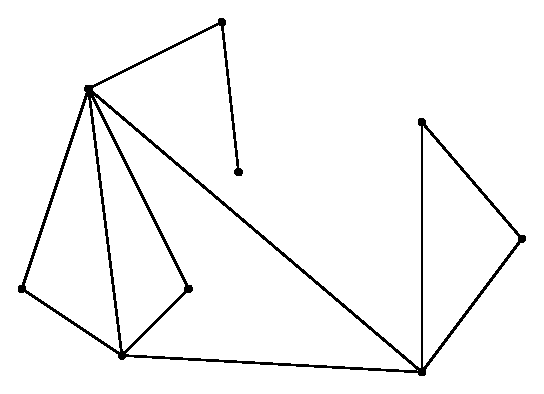
\includegraphics[width=0.7\textwidth]{3_1.eps}\\
  \caption{}
\end{figure}
\end{defination}
\begin{theorem}
$e=(u,v)$是割边,当且仅当e不属于G的任何回路。\\
\textbf{证明:}\\
\begin{itemize}
  \item 充分性(反证法):若$e=(u,v)$属于G的某个回路,则$G'=G-e$中仍存在u到v的道路,故结点u和v属于同一连通支,e不是割边。
  \item 必要性(反证法):反之,若e不是割边,则$G'$和G
的连通支数一样,因此u和v仍然处在同一个连
通支,因此在图$G'$中存在道路$P(u,v)$ $$P(u,v)+e$$就是图G的一个回路.
\end{itemize}
\end{theorem}
\begin{theorem}
$e=(u,v)$是割边,当且仅当e不属于G的任何回路。\\
\end{theorem}
\textbf{小结论:}
\begin{itemize}
  \item \textcolor{red}{树的每条边都不属于任何回路}
  \item \textcolor{red}{因此树的每条边都是割边}
  \item \textcolor{red}{树是边数最少的连通图}
\end{itemize}
\subsection{树的等价性质}
\begin{theorem}
设T 是结点数为$n\geq2 $的树, 则下列性质等价:
\begin{enumerate}
  \item T连通且无回路
  \item T 连通且每条边都是割边
  \item T连通且有n-1 条边
  \item T 有n-1 条边且无回路
  \item T的任意两结点间有唯一道路
  \item T 无回路,但在任意两结点间加上一条边后恰有一个回路
\end{enumerate}
{\hwxw 依次证明上述定理的正确性:}
{\song
\begin{itemize}
  \item (1)T连通且无回路$\Rightarrow$(2)T连通且每条边都是割边\\
  \textbf{证明:}\\
  由定理$3.1.2$ ,$e=(u,v)$是割边$\Leftrightarrow$ e 不属于G的任何回路.
  \item (2)T 连通且每条边都是割边$\Rightarrow$ (3)T 连通且有n-1 条边\\
  \textbf{证明:}\\
  采用数学归纳法: 对结点数n 进行归纳。\\
  设m(T) 为树T 的边数,n(T) 为树T 的结点数。\\
  n=2 时, 结论显然成立;\\
  设$n\leq k$ 时,$m(T)=n(T)-1$ 成立。\\
  当$n=k+1$ 时, 由于每条边都是割边, 因此图$G'=G - e$ 有两个连通支$T_1$和$T_2$。\\
  根据假设,$$ m(T_1)=n(T_1)-1,\quad m(T_2)=n(T_2)-1 \Rightarrow $$ $$m(T)=m(T_1)=m(T_2)+1=n(T)-1$$
  \item (3)T 连通且有$n-1$条边$\Rightarrow$(4)T 有$n-1$ 条边且无回路 \\
  \textbf{证明:}\\
  反证法: 假定T 有回路。\\
    设C 为其中一条含有k 个结点的初级回路,故回路内有k 条边。考察C 以外的$n-k $个结点, 为保持T 的连通性, 至少需要C 以外的n-k 条
    边。所以T 的边数至少为$k+(n-k)=n$ 条与T 有$n-1$ 条边矛盾,故假设不成立,即T 无回路。
  \item(4) T有$n-1$ 条边且无回路$\Rightarrow$ (5)T 的任意两结点间有唯一道路\\
  \textbf{证明:}\\
  首先证明任意两结点间道路的存在性(反证法) : 设$u,v$ 是T 的任
意两结点, 假设不存在道路$P(u,v)$ 则$u,v$ 属于两个连通支$T_1,T_2$。 由于$m=n-1$, 则至少有一个连通支的边数不少于结点数。不妨
设为$T_1,m(T_1)\geq n(T_1)$ 设$T_1$ 无回路,由性质(1)$\Rightarrow$ 性质(2)
$\Rightarrow$性质(3),$m(T_1)=n(T_1)-1<n(T_1)$,矛盾。因此此时该连通支
$T_1$ 必存在回路, 与题目前提矛盾! 因此, $P(u,v)$ 存在。\\
其次证明任意两结点间道路的唯一性:\\
如图$3.2$, 若存在两条不同的道路$P(u,v), P'(u,v)$,则$P(u, v)\bigoplus P'(u, v)$
必存在回路。与题目假设矛盾。因此$P(u,v)$ 唯一。
\begin{figure}[H]
  \centering
  % Requires \usepackage{graphicx}
  \includegraphics[width=0.6\textwidth]{3.2.png}\\
  \caption{}
\end{figure}
\item (5)T的任意两结点间有唯一道路$\Rightarrow \quad $ (6)T 无回路, 但在任意两结点间
加上一条边后恰有一个回路\\
\textbf{证明:}\\
 首先证明T 无回路:\\
若T 有回路,则回路上任意两点之间至少有两条不同的道路,与
前提矛盾。\\
故T 无回路。\\
 其次证明在任意两结点间加上一条边e 后恰有一个回路:\\
设原来两结点之间的道路为P,则$P\bigcup e $即为一个回路。\\
故在任意两结点间加上一条边e 后恰有一个回路\\

\item (6)T 无回路, 但在任意两结点间加上一条边后恰有一个回路$\Rightarrow \quad$ (1)T
连通且无回路\\
\textbf{证明:}
 T 连通:因任意两结点间加上一条边后恰有一个回路,故原图中
任意两点间必然存在一条道路。\\
T 无回路:已知条件
\end{itemize}
}
\end{theorem}
\begin{theorem}
树T中一定存在树叶结点\\
{\song
\textbf{证明:}\\
T为连通图,故不存在度为零的结点。\\
假设T中不存在树叶结点,则意味着不存在度为
1的结点,则所有结点度均不小于2。
$$ m=\frac{1}{2}\sum_{v\in V(G)} d(v)\quad \Rightarrow \quad m \geq \frac{1}{2}\cdot 2n=n > n-1$$
容易看出:矛盾!\\
}
\end{theorem}
\begin{defination}
如果T是图G的支撑子图,而且又是一棵树,则称T是G的一棵\textcolor{red}{支撑树},或称\textcolor{red}{生成树},又简称为G的\textcolor{red}{树}。
\end{defination}
\subsection{余树的概念}
\begin{defination}
G中删掉T的各边后子图称为T的\textcolor{red}{余树},记为$\bar{T}$
\end{defination}

\section{基本关联矩阵及其性质}
{\hwxw 本节研究的范围是有向连通图。}\\
\begin{defination}
有向连通图$G = (V , E)$ 的关联矩阵$B $中划去任意节点$v_k$ 所
对应的行,得到一个$(n−1)\times m$ 的矩阵$B_k$, $B_k$ 称为G 的一个基本关联矩阵。
\begin{figure}[H]
  \centering
  % Requires \usepackage{graphicx}
  \includegraphics[width=0.6\textwidth]{3_3.eps}\\
  \caption{}
\end{figure}
\begin{equation}
B=\bordermatrix{%
       & e_1       & e_2     &e_3    &e_4  &e_5 &e_6\cr
v_1    & 1         & -1       &1     & 0 & 0 & 1\cr
v_2    & 0        & 0       &-1     & -1 & 0 & -1\cr
v_3    & -1         & 1       &0     &0 &1 &0
},
\end{equation}
\end{defination}
{\hwxw 下面我们来研究基本关联矩阵的性质。\\}
\begin{theorem}
有向图$G = (V , E)$ 关联矩阵B 的秩$ran(B) < n$。\\
{\song
\textbf{证明:}\\
关联矩阵特点:每一列都只有一个$1$和$-1$\\
n行全部相加\\
即n 个行向量线性相关,因此
$$ran B< n$$
证毕!
}
\end{theorem}
\begin{theorem}
设$B_0$是有向图G关联矩阵B的任意一k阶子方阵,则$det(B_0)$为$0,1$或$-1$\\
{\song
\textbf{证明:}\\
若$B_0$某列全零,则$det(B_0)=0$\\
若$B_0$每列都有两个非零元,则$det(B_0)=0$\\
若$B_0$存在某列只有一个非零元,则按该列展开可知$det(B_0)=\pm det(B_1)$\\
依次类推,可证!
}
\end{theorem}

\begin{theorem}
设$B_0$是有向图G关联矩阵B的任意一k阶子方阵,则$det(B_0)$为$0,1$或$-1$\\
{\song
\textbf{证明:}\\
若$B_0$某列全零,则$det(B_0)=0$\\
若$B_0$每列都有两个非零元,则$det(B_0)=0$\\
若$B_0$存在某列只有一个非零元,则按该列展开可知$det(B_0)=\pm det(B_1)$\\
依次类推,可证!
}
\end{theorem}

\begin{theorem}
设B是有向连通图G的关联矩阵,则$$ran B=n-1$$
{\song
\textbf{证明:}\\
设B中最少的线性相关行数为$l$\\
则$l\leq n$,其对应图中结点$v(i_1),v(i_2),\dots,v(i_l )$\\
\begin{equation*}
k_1\cdot b(i_1) +k_2\cdot b(i_2) +\cdots +k_l\cdot b(i_l) =O_m \quad (k_j\neq 0,\quad j=1,2,\cdots,l)
\end{equation*}
\begin{itemize}
  \item
  \begin{center}
    所有$b(i_j)$中,第$t(t=1,2,\cdots m)$个分量可能
  \end{center}
  \item
  \begin{center}
    所有$b(i_j)$中,第$t(t=1,2,\cdots m)$个分量可能
  \end{center}
  \item
  \begin{center}
    所有$b(i_j)$中,第$t(t=1,2,\cdots m)$个分量不可能
  \end{center}
\end{itemize}
  \begin{flushleft}
    否则,该分量最终不可能为$0$。
\end{flushleft}
\quad 这样,我们可以对矩阵B进行行、列交换,使前$l$行为线性相关的各行\\
\quad 再针对这$l$ 行中,有两个非零元的列换到前$r$列\\
则此$l$ 行中,其余$(m-r)$列将均为零元\\
\quad 此时矩阵B将变为
\begin{align*}
 B'= \begin{array}{lc}
\mbox{}&
\begin{array}{cc}r&m-r \end{array}\\
\begin{array}{c}l\\n-l\end{array}&
\left[\begin{array}{cc}
P&0\\
0&Q
\end{array}\right]
\end{array}
\quad \quad ran B=ran B'
\end{align*}
\quad 若$l <n$,则从$B'$可清楚看出,图G为两个连通支,这与
图G为连通图矛盾!\\
因此,一定有$l=n$
}
\end{theorem}
\begin{theorem}
设B是有向连通图G的关联矩阵,则$$ran B=n-1$$
\end{theorem}
\begin{theorem}
连通图G基本关联矩阵$B_k$的秩$$ran B_k=n-1$$
\end{theorem}
\begin{theorem}
设$B_k$为有向连通图G的基本关联矩阵,C为G中的一个回路。则C中各边所对应$B_k$的各列线性相关。\\
{\song
\textbf{证明:}\\
只需针对C为初级回路进行讨论即可\\
设C中含$l$个结点与$l$条边$(l<n)$,这$l$条边对应关联矩阵$B$中的$l$列,它们构成子阵$B(G_C)$  \\
\begin{figure}[H]
  \centering
  % Requires \usepackage{graphicx}
  \includegraphics[width=0.7\textwidth]{3.4.png}\\
  \caption{}
\end{figure}
\noindent C的关联矩阵为$l$ 阶方阵$B(C)$,据定理$3.2.5$ $$ran B(C)=l-1$$
说明$B(C)$的$l$列线性相关\\
观察$B(C)$与$B(G_C)$的关系:
{\hwxw
\begin{itemize}
  \item B(C)为$B(G_C)$的子阵,列数相同,行数不同
  \item C中各边只经过B(C)中的各结点,因此$B(G_C)$中其他结点对应各
行均为零
\end{itemize}
}
因此, $B(G_C)$的各列也线性相关!\\
因此,在$B_k$中,C对应各列也线性相关!\\
}
\end{theorem}
\begin{theorem}
设$B_k$为有向连通图G的基本关联矩阵,C为G中的一个回路。则C中各边所对应$B_k$的各列线性相关。\\
\end{theorem}
\begin{coro}
设H为连通图G的子图,如果H含有回路,
则H的\textcolor{red}{诸边}对应的G的基本关联矩阵各列线性相关。
\begin{figure}[H]
  \centering
  % Requires \usepackage{graphicx}
  \includegraphics[width=0.4\textwidth]{rank.png}\\
  \caption*{}
\end{figure}
\end{coro}
{\hwxw
思考:\\
有向连通图的基本关联矩阵,哪些列线性相关?\\
有向连通图的基本关联矩阵,哪些列线性不相关?\\
}
\begin{theorem}
令$B_k$是有向连通图G的基本关联矩阵,那么$B_k$的任意$n-1$阶子阵行列式非零的充要条件是其各列所对应的边构成G的一棵支撑树。
{\song
证明:\\
充分性:\\
设T为G的支撑树\\
子图T的基本关联矩阵$B_k(T)$是$n-1$阶子方阵,它的秩为$n-1$这意味着其行列式非零。\\
该子方阵恰好就是$B_k$的某个$n-1$阶子阵\\
即$B_k$所对应的该$n-1$阶行列式非零。\\
}
\end{theorem}
\begin{shaded}
{\hwxw
小结:\\
(1)有向连通图关联矩阵的秩\\
(2)有向连通图基本关联矩阵各列的线性相关性\\
(3)有向连通图基本关联矩阵同支撑树的关系\\
}
\end{shaded}

\section{支撑树的计数}
给定连通图G,其支撑树可以有多少个?\\
以某结点为根的支撑树可以有多少个?
\begin{figure}[H]
  \centering
  % Requires \usepackage{graphicx}
  \includegraphics[width=0.5\textwidth]{3_5.eps}\\
  \caption*{}
\end{figure}
\begin{theorem}
(Binet-Cauchy定理)已知两个矩阵$A=(a_{ij})_{m\times n}$
和$B=(b_{ij})_{n\times m}$,满足$m\leq n$,则$$ det(AB)=\sum_{i}(A_iB_i)$$
{\hwxw
其中$A_i$,$B_i$都是m阶行列式\\
$A_i$是从A中取不同的m列所成的行列式;\\
$B_i$是从B中取相应的m行构成的行列式;\\
结果为全部组合求和\\
}
\end{theorem}
\begin{sample}
已知$A=\left[
       \begin{array}{ccc}
         4 & 3 & 2 \\
         -2 & 4 & 3 \\
       \end{array}
     \right]
$\quad $B=\left[
           \begin{array}{cc}
             5 & 1 \\
             0 & 3 \\
             4 & 2 \\
           \end{array}
         \right]
$求$det(AB)$\\
解:\\
$AB=\left[
      \begin{array}{cc}
        28 & 17 \\
        2 & 16 \\
      \end{array}
    \right]
$\\
因此$det(AB)=28 \times 16-17\times 2=414$\\
\end{sample}
\begin{shaded}
\noindent 采用内比-柯西定理计算矩阵乘积的行列式通常比较复杂\\
其价值在于:揭示了乘积矩阵的行列式与各矩阵的子阵行列式之间的关系\\
连通图中不同支撑树的计数恰好利用了这种关系,从而可以用代数的方法很容易解决支撑树的计数问题
\end{shaded}
\subsection{支撑树的计数-有向连通图}
\begin{theorem}
设$B_k$的是有向连通图$G=(V,E)$的某一
基本关联矩阵,则G的不同树的数目是$$det(B_kB^T_k)$$
{\song
证明:设$B_k=(b_{ij})_{(n-1)\times m}$\\
由内比-柯西定理$$det(B_k B_k^T)=\sum_{i}|B_i||B_i^T|$$
其中$|B_i|$是$B_k$的某$n-1$阶子阵的行列式\\
$|B_i^T|$是对应的$B_i^T$的$n-1$阶阵的行列式\\
有$|B_i|=|B_i^T|$\\
因此可以得到$$det(B_k B_k^T)=\sum_{i}|B_i||B_i^T|=\sum_i|B_i|^{2}$$
由定理$3.2.9$,如果,则其所对应的边构成G的一棵树\\
再由定理$3.2.3$, $|B_i|$只能为$0,1$或$-1$\\
因此, $det(B_k b_k^T)$恰恰是G中不同树的数目\\
}
\end{theorem}
\begin{sample}
如图$3.5$
\begin{figure}[H]
  \centering
  % Requires \usepackage{graphicx}
  \includegraphics[width=0.5\textwidth]{3_5_1.eps}\\
  \caption{}
\end{figure}
$
B=\left[
    \begin{array}{ccccccc}
      v_1 & 1 & -1 & 1 & 0 & 0 & 1 \\
      v_2 & 0 & 0 & -1 & -1 &0 & -1 \\
      v_3 & -1 & 1 & 0 & 0 & 1 & 0 \\
      v_4 & 0 & 0 & 0 & 1 & -1 & 0 \\
      & e_1 & e_2 & e_3 & e_4 & e_5 & e_6 \\
    \end{array}
  \right]\quad \Rightarrow \quad
  B_4=\left[
    \begin{array}{ccccccc}
      v_1 & 1 & -1 & 1 & 0 & 0 & 1 \\
      v_2 & 0 & 0 & -1 & -1 &0 & -1 \\
      v_3 & -1 & 1 & 0 & 0 & 1 & 0 \\
      v_4 &  &  &  &  &  & \\
      & e_1 & e_2 & e_3 & e_4 & e_5 & e_6 \\
    \end{array}
  \right]
$ $$det(B_4 B_4^T=8)$$
\end{sample}
\subsection{含特定、不含特定边的计算方法}
\begin{enumerate}
  \item 计算G 中不含某特定边$e$ 的树的数目:
将该边删除即可!
  \item 计算G 中必定含特定边e 的树的数目:
将该边收缩即可!
\end{enumerate}
\section{无向连通图支撑树的计数}
{\hwxw 无向连通图的关联矩阵不存在-1 元素, 如何计算其支撑树的数目?}\\
对无向连通图G 的每边任给一个方向, 得到有向连通图$G'$, 则$G'$的
支撑树与G 的支撑树一一对应!\\
\section{有向连通图根树的计数}
\begin{defination}
根树:T 为有向树, 若T 中存在某结点v0 的负度为0, 其余结点负
度为1, 则称T 为以$v_0$ 为根的外向树, 或称根树, 用$\mathop{T}\limits^{\rightharpoonup}$ 表示。
例:
\begin{figure}[H]
  \centering
  % Requires \usepackage{graphicx}
  \includegraphics[width=0.5\textwidth]{3_6.eps}\\
  \caption*{}
\end{figure}
$\Rightarrow \quad B_0=\left[
                         \begin{array}{ccccc}
                           v_0 &  &  &  &  \\
                           v_1& -1 & 0 & 1 & 1\\
                           v_2 & 0 & 0 & -1 & 0 \\
                           v_3 & 0 & 0 & 0& -1 \\
                           v_4 & 0 & -1 & 0 & 0 \\
                          & e_1  & e_2 & e_3 & e_4 \\
                         \end{array}
                       \right]
$\\
{\hwxw 特点:除$v_0$外,每行只有一个$-1$}\\
\subsection{根树基本关联矩阵的性质和特点}
如果对根树的结点和边重新进行编号,使
每条边$e=(v_i,v_j)$都满足$v_i$的编号小于$v_j$的编号,
同时$e=(v_i,v_j)$的编号为$e_j$
\begin{figure}[H]
  \centering
  % Requires \usepackage{graphicx}
  \includegraphics[width=0.5\textwidth]{3_7.eps}\\
  \caption*{}
\end{figure}
$\Rightarrow \quad B_0'=\left[
                         \begin{array}{ccccc}
                           v_1& -1 & 0 & 0 & 0\\
                           v_2 & 0 & -1& 1 & 1 \\
                           v_3 & 0 & 0 & -1& 0 \\
                           v_4 & 0 & 0 & 0 & -1 \\
                          & e_1  & e_2 & e_3 & e_4 \\
                         \end{array}
                       \right]
$\\
{\hwxw 思考:为什么按照规则编号后,根树中根结点对应的
基本关联矩阵一定是上三角矩阵?\\}
\end{defination}
\begin{shaded}
特点:按照规则编号后, 根树中根结点对应的基本关联矩阵一定是上三
角矩阵。\\
非根树基本关联矩阵可调整为上三角矩阵, 且对角线上将出现“1”元素。\\
令${\mathop{B}\limits^{\rightharpoonup}}_k$ 表示有向连通图G 的基本关联矩阵$B_k$ 中全部1 元素改为0 后的
矩阵。相应地,G 的支撑树的基本关联矩阵, 可调整为上三角矩阵, 但原先的
“1”变为了“0”。\\
\indent 如果该树为非根树(行列式为零), 则对角线将出现“0”元素\\
\indent 如果该树为根树(行列式绝对值为“1”), 则对角线全部为“-1”元素
\end{shaded}
\subsection{根树的计算方法}
\textbf{回顾:}定理$3.3.2$\\
设$B_k$的是有向连通图$G=(V,E)$的某一
基本关联矩阵,则G的不同树的数目是$$det(B_kB^T_k)$$
\begin{theorem}
有向连通图G 中以$v_k$ 为根的根树数目是$$det(\mathop{B_k}\limits^{\rightharpoonup}B_k^T)$$
{\song
证明:\\
由比内-柯西定理$$det(\mathop{B_k}\limits^{\rightharpoonup}B_k^T)=\sum_{i}|\mathop{B_i}\limits^{\rightharpoonup}||B_i^T|$$
若$|B_i^T|\neq 0$, 说明这$n-1$ 条边构成了G 的一棵树\\
若$ \mathop{B_i}\limits^{\rightharpoonup} \neq 0$, 说明该树是以$v_k$ 为根的根树。\\
二者的乘积非零说明存在一棵vk 为根的根树。
由于遍历了所有$n-1$ 条边的组合, 因此$$det(\mathop{B_k}\limits^{\rightharpoonup}B_k^T)=\sum_{i}|\mathop{B_i}\limits^{\rightharpoonup}||B_i^T|$$
为以$v_k$ 为根的根树的数目
}
\end{theorem}
\subsection{含特定边、不含特定边的根树计算方法}
1. 如何计算以v0 为根结点不含某特定边e 的根树的数目?\\
\indent 作$G'=G-e$,计算$G'$的以$v_0$ 为根结点的根树的数目即可\\
2. 如何计算以$v_0$ 为根结点必含某特定边e 的根树的数目?\\
\begin{itemize}
  \item 将该边收缩为一点\\
\textcolor{red}{错误!}此方法未必得到根树!
  \item 先计算以$v_0$ 为根结点的根树数目, 再计算不含边e 的根树数目,
求差值即可。
  \item 其他计算方法:
设$e=(u, v)$, 将除e 之外所有以v 为终点的边都删掉得到$G'$, 然
后计算$G'$的以$v_0$ 为根结点的根树的数目即可
\end{itemize}
\section{回路矩阵与割集矩阵}
\subsection{回路矩阵及其性质}
设T是有向连通图$G=(V,E)$的一棵支撑树,对
任意边$e\in E(G)-E(T)$,$T+e$ 都可构成G的一
个唯一回路C。给定回路C一个参考方向,
则C中的边如和方向一致,称之为\textcolor{red}{正向边},
否则称之为\textcolor{red}{反向边}。\\
\begin{defination}
有向连通图G的全部初级回路构成
的矩阵,称为G的\textcolor{red}{完全回路矩阵},记为$C_e$ :
\begin{equation*}
  c_{ij}=\begin{cases}
1 & ,e_j\in C_i \text{且与回路}C_i\text{方向一致}\\
-1 & ,e_i\in C_i \text{且与回路}C_i \text{方向相反}\\
0 &,\text{其他}
\end{cases}
\end{equation*}
例:\\
\begin{figure}[H]
  \centering
  % Requires \usepackage{graphicx}
  \includegraphics[width=0.8\textwidth]{ce.png}\\
  \caption*{}
\end{figure}
\end{defination}
\begin{shaded}
{\hwxw 思考:图G中会有多少个初级回路?}\\
给定G的一个支撑树T,理论上最多可以生成$2^{m-n+1}-1$个初级回路。
\begin{itemize}
  \item T有$n-1$条边,则余树有$m-n+1$条边
  \item T中加入余树中任意几条边都有可能构成初级回路
  \item $m-n+1$条边每条边都有两种选择,但不能一条边都没有
\end{itemize}
\end{shaded}
\begin{defination}
当有向图$G=(V,E)$的支撑树T确定后,每条余树边e所对应的回路称为基本回路,该回路的方向与e的方向一致。由全部基本回路构成的矩阵称为G的\textcolor{red}{基本回路矩阵},记为$\mathbf{C_f}$\\
例:
\begin{figure}[H]
  \centering
  % Requires \usepackage{graphicx}
  \includegraphics[width=0.8\textwidth]{cf.png}\\
  \caption*{}
\end{figure}
$C_f=(I,C_{f_{12}})$\\
\textcolor{red}{显然,基本回路矩阵的秩为$m-n+1$}
\end{defination}
\begin{theorem}
有向连通图$G=(V,E)$的关联矩阵B和
完全回路矩阵$C_e$的边次序一致时,恒有:$$BC^T_e=0$$
{\song
证明:设$D=BC^T_e$,则$$d_{ij}=\sum_{k=1}^{m}b_{ik}\cdot c_{jk}$$
其中$b_{ik}$是结点$v_i$和边$e_k$的关联情况\\
$c_{jk}$是回路$c_j$和边$e_k$的关联情况\\
\textbf{回路$C_j$与结点$v_i$只有两种情况:}\\
\textcolor{red}{第一种}:$C_j$不经过结点$v_i$:\\
$\bullet$ 与$v_i$关联的任一边都不是$C_j$中的边\\
$\bullet$ 此时$b_{ik}$不为零时,$c_{jk}$一定为零\\
$ \bullet$ $c_{jk}$不为零时,$b_{ik}$一定为零
\begin{figure}[H]
  \centering
  % Requires \usepackage{graphicx}
  \includegraphics[width=0.5\textwidth]{f1.png}\\
  \caption*{}
\end{figure}
$$d_{ij}=\sum_{k=1}^{m}b_{ik}\cdot c_{jk}=0$$
\textcolor{red}{第二种}:$C_j$经过结点$v_i$\\
$\bullet$ 则$C_j$必定经过与$v_i$关联的两条边$e_p$和$e_q$\\
$\bullet$ 若$e_p$和$e_q$同向,则$C_{jp}$和$C_{jq}$同正负,$b_{ip}$和$b_{iq}$一正一负\\
$\bullet$ 若$e_p$和$e_q$反向,则$c_{jp}$和$c_{jq}$一正一负,$b_{ip}$和$b_{iq}$同正负
\begin{figure}[H]
  \centering
  % Requires \usepackage{graphicx}
  \includegraphics[width=0.5\textwidth]{f2.png}\\
  \caption*{}
\end{figure}
$$d_{ij}=\sum_{k=1}^{m}b_{ik}\cdot c_{jk}=0$$
$$BC_{e}^{T}=0$$
}
\end{theorem}
\begin{coro}
有向连通图的基本关联矩阵$B_k$,基本回路矩阵$C_f$ ,在边次序一致的情况下,有$$B_kC_f^T=0$$
\end{coro}
\begin{theorem}
若有向连通图$G=(V,E)的$基本关联
矩阵$B_k$是和基本回路矩阵$C_f$ 的边次序一致,并设$C_f=(I \quad C_{f_{12}}) \quad ,B_k=(B_{11} \quad B_{12}),$
$$ C_{f_{12}}=-B_{11}^T\cdot(B_{12}^{-1})^T$$
{\song
证明:\\
由推论知$B_kC^T_f=0$,写成块矩阵形式
\begin{equation*}
(B_{11},B_{12})\left[
                 \begin{array}{c}
                   I \\
                   C_{f_{12}}^T \\
                 \end{array}
               \right]=0\quad \quad \Rightarrow \quad B_{12}\cdot  C_{f_{12}}^T=-B_{11}
\end{equation*}
}
\end{theorem}
\begin{shaded}
定理$3.6.2$说明了基本关联矩阵和基本回路矩阵之间的关系\\
\indent 说明根据基本关联矩阵,可以通过计算得到基本回路矩阵
如果$B_k$已知,而且确定了一棵树,则可以直接经过计算求出G的基本回路矩阵$C_f$。
\end{shaded}
\begin{sample}
\begin{figure}[H]
  \centering
  % Requires \usepackage{graphicx}
  \includegraphics[width=0.5\textwidth]{dianlu.png}\\
  \caption*{一个电路网络}
\end{figure}
已知上图基本关联矩阵\\
$B_4=
\begin{array}{c}
%\mbox{}&
\begin{array}{cccccc}e_1&e_2&e_3&e_4&e_5&e_6 \end{array}\\
%\begin{array}{c}\\ \end{array}&
\left[\begin{array}{cccccc}
1&-1&1&0&0&0\\
0&1&0&-1&0&-1\\
-1&0&0&1&1&0
\end{array}\right]
\end{array}
$
其中$e_1,e_5,e_6$所对应的子阵行列式非零,求$C_f$。\\
解:由$e_1,e_5,e_6$可以构成G的一棵树。对$B_4$进行行列式交换得到\\
$
B_4=
\begin{array}{c}
%\mbox{}&
\begin{array}{cccccc}e_1&e_2&e_3&e_4&e_5&e_6 \end{array}\\
%\begin{array}{c}\\ \end{array}&
\left[\begin{array}{cccccc}
-1&1&0&1&0&0\\
1&0&-1&0&0&-1\\
0&0&1&-1&1&0
\end{array}\right]
\end{array}=(B_{11} \quad B_{12})
$\\
因此$C_{f_{12}}=-B_{11}^TB_{12}^{-T}=\left[
                                     \begin{array}{ccc}
                                       1 & 1 & 1 \\
                                       -1 & -1 & 0 \\
                                       0 & -1 & -1 \\
                                     \end{array}
                                   \right]
$\\
$B_{11}=\left[
        \begin{array}{ccc}
          -1 & 1 & 0 \\
          1 & 0 & -1 \\
          0 & 0 & 1 \\
        \end{array}
      \right] \quad B_{12}=\left[
        \begin{array}{ccc}
          1 & 0 & 0 \\
          0 & 0 & -1 \\
          -1 & 1 & 0 \\
        \end{array}
         \right] \quad B_{12}^{-1}=\left[
        \begin{array}{ccc}
          1 & 0 & 0 \\
          1 & 0 & -1 \\
          0 & 1 & 0 \\
        \end{array}
         \right]
$\\
即$$C_f=\begin{array}{c}
%\mbox{}&
\begin{array}{cccccc}e_1&e_2&e_3&e_4&e_5&e_6 \end{array}\\
%\begin{array}{c}\\ \end{array}&
\left[\begin{array}{cccccc}
1&0&0&1&1&1\\
0&1&0&-1&-1&0\\
0&0&1&0&-1&1
\end{array}\right]
\end{array}$$
\end{sample}
\begin{theorem}
有向连通图$G=(V,E)$完全回路矩阵
的秩为$(m-n+1)$\\
{\song
基本回路矩阵为完全回路矩阵的子阵(列数相
等,行数不等)。\\
基本回路矩阵秩为$m-n+1$\\
则完全回路矩阵的秩不小于$m-n+1$\\
即:$$ran(C_e)\geq m-n+1$$
sylvester定理: 设A,B分别为$n\times m$与$m\times s$的
矩阵,则$ran (AB) \geq ran (A)+ran (B)-m$
\begin{gather*}
                                       B:n\times m \quad ran(B)=n-1 \\
                                       C_e^T:m \times s \quad ran(C_e^T)=?\\
                                       BC_e^T=0 \quad \Rightarrow \quad ran(BC_e^T)=0
                                     \end{gather*}
 即:$ran(C_e^T)\leq m-n+1$\\
 故:$ran(C_e)=m=n+1$

}
\end{theorem}
\begin{defination}
有向连通图G中$(m-n+1)$个互相独立的回路组成的矩阵,称为G的\textcolor{red}{回路矩阵},
记为C。
\end{defination}
\begin{shaded}
\noindent 回路矩阵C具有以下几个简单性质:\\
(1).基本回路矩阵$C_f$ 是回路矩阵\\
(2).$BC^T=0$,其中B与C的边次序一致\\
(3). $C=P\cdot C_f$,其中P为非奇异方阵,C与$C_f$ 边次序
一致
\end{shaded}

\begin{theorem}
连通图$G=(V,E)$的回路矩阵C的任一$(m-n+1)$阶子阵行列式非零,当且仅当这些列对应于G的某一棵余树\\
{\song
证明:\\
\textcolor{red}{充分性}:已知余树$\bar{T}$ $\quad \Rightarrow \quad $对应行列式非零\\
可构造出G的基本回路矩阵$C_f=(I \quad C_{f_{12}})$。\\
 对给定的回路矩阵C进行列交换,使其边序与$C_f$
一致,这样可写为$C=(C_{11} \quad C_{12})$,其中$C_{11}$对应
余树$\bar{T}$\\
由性质(3)$C=P\cdot C_f$ ,即$$ (C_{11} \quad C_{12})=P(I \quad C_{f_{12}})=(P \quad P\cdot C_{f_{12}})$$
因此,$C_{11}=P$,P非奇异,即$C_{11}$行列式非零\\
\\
\textcolor{red}{必要性:}已知回路矩阵C的某($m-n+1)$阶子阵行列式非零。\\
将这$(m-n+1)$列放在前面,写为$C=(C_{11} \quad C_{12})$\\
求证$C_{11}$对应的是一棵余树(反证法):\\
假设$C_{12}$对应的不是一棵树,则$C_{12}$中必含回路,不妨设为$C_x$\\
由于回路矩阵的各行线性无关,且完全回路矩阵秩为$m-n+1$\\
{\hwxw \textcolor{red}{任意一个回路都可以由回路矩阵各行向量线性表示!}}\\
因此,$C_x$一定可以由C中各行线性表示,即C经
过行初等变换,可以得到表示$C_x$的行向量
\begin{equation*}
  C=(C_{11}\quad C_{12}) \quad \Rightarrow \quad C'=\left[
                                                      \begin{array}{cc}
                                                        C_{11}' & C_{12}' \\
                                                       \qquad  \quad C_x \\
                                                      \end{array}
                                                    \right]\quad \Rightarrow \quad
                                                    C'=\left[
                                                      \begin{array}{cc}
                                                        C_{11}' & C_{12}' \\
                                                        0 & C_{12}'' \\
                                                      \end{array}
                                                    \right]
\end{equation*}
即$C_{11}$可经过行初等变换,可得到\\
说明$C_{11}$行列式为零,与前提矛盾。\\
因此$C_{12}$对应的是一棵树,$C_{11}$对应其余树!\\
}
\end{theorem}

\begin{theorem}
令$B_k$是有向连通图G的基本关联矩阵,那么$B_k$的任意$n-1$阶子阵行列式非零的充要条件是其各列所对应的边构成G的一棵支撑树。\\
\end{theorem}

\subsection{割集矩阵及其性质}
\begin{defination}
设S为有向图$G=(V,E)$的边子集,若:\\
$1.$ $G'=(V,E-S)$比G的连通支数多$1$\\
$2.$ 对任意S的真子集$S'$,$G''=(V,E-S')$与G的连通支数相同\\
则称S为G的一个\textcolor{red}{割集}\\
一般给割集S一个方向,称它为\textcolor{red}{有向割集}\\
\end{defination}

\begin{defination}
有向连通图G的全部割集构成的矩
阵,称为G的完全割集矩阵,记为$S_e$:
$$S_{ij}=\begin{cases}
1 &,e_j\in S_i \text{且与割集}S_i \text{方向一致}\\
-1&,e_j\in S_i \text{且与割集}S_i \text{方向相反}\\
0&,\text{其他}
\end{cases}
$$
例:\\
\begin{figure}[H]
  \centering
  % Requires \usepackage{graphicx}
  \includegraphics[width=0.8\textwidth]{f3.png}\\
  \caption*{}
\end{figure}
\end{defination}

\begin{shaded}
{\hwxw 思考:图G中会有多少个割集?}\\\begin{itemize}
                          \item[-]一个割集可将连通图分为两个部分,连通图的一个划分就对应一个割集
                          \item[-] n个结点划分为两个部分,有多少种分法?
                          \item[-]设想将n个不同的球放入两个盒子$$\frac{2^n-2}{2}=2^{n-1}-1$$
                        \end{itemize}
\textbf{完全割集矩阵规模为$(2^{n-1}-1)\times m$}
\end{shaded}

\begin{defination}
设T是连通图G 的一棵树,$e_i$ 是树枝。对应$e_i$ 存在G的割集$S_i$,$S_i$只包括一条树枝$e_i$ 及某些余树枝,且与$e_i$ 的方向一致。此时称$S_i$ 为G的对应树T 的一个\textcolor{red}{基本割集}\\
\end{defination}

\begin{defination}
给定有向连通图G的一棵树T,由对应T的全部基本割集组成的矩阵称为\textcolor{red}{基本割集矩阵},记为
$\mathbf{S_f}$\\
例:
\begin{figure}[H]
  \centering
  % Requires \usepackage{graphicx}
  \includegraphics[width=0.8\textwidth]{f4.png}\\
  \caption*{}
\end{figure}

\end{defination}

\begin{theorem}
当有向连通图G的完全回路矩阵$C_e$和完全割集矩阵$S_e$的边次序一致时,有
$$S_eC_e^T=0$$
{\song
证明:设$D=S_eC_e^T$,则$$d_{ij}=\sum_{k=1}^{m}s_{ik}\cdot c_{jk}$$
其中$S_{ik}$是第i 个割集$S_i$中的情况\\
\indent $c_{jk}$是第j个回路$c_j$中的情况\\
\textcolor{red}{回路$C_j$与割集$S_i$只有两种情况:\\}
\textbf{第一种情况:}$C_j$与割集$S_i$无公共边(不相交):\\
\begin{figure}[H]
  \centering
  % Requires \usepackage{graphicx}
  \includegraphics[width=0.5\textwidth]{f5.png}\\
  \caption*{}
\end{figure}
\noindent $\bullet$此时$S_i$中的任一边都不是$C_j$中的边\\
$\bullet$此时$s_{ik}$不为零时,$c_{jk}$一定为零\\
$\bullet$ $c_{jk}$ 不为零时, $s_{ik}$一定为零\\
$$d_{ij}=\sum_{k=1}^{m}s_{ik}\cdot c_{jk}=0$$
\textbf{第二种情况:}$C_j$与割集$S_i$有公共边(相交):\\
\begin{figure}[H]
  \centering
  % Requires \usepackage{graphicx}
  \includegraphics[width=0.5\textwidth]{f6.png}\\
  \caption*{}
\end{figure}
\noindent $\bullet$则$C_j$必定与$S_i$\textcolor{red}{有成对出现的}偶数条公共边$e_p$和$e_q$\\
$\bullet$若$e_p$和$e_q$同向,则$c_{jp}$和$c_{jq}$一正一负,$s_{ip}$和$s_{iq}$同正负\\
$\bullet$ 若$e_p$和$e_q$反向,则$c_{jp}$和$c_{jq}$同正负,$s_{ip}$和$s_{iq}$一正一负\\
$$d_{ij}=\sum_{k=1}^{m}s_{ik}\cdot c_{jk}=0$$
$$S_eC_e^T=0$$
}
\end{theorem}

\begin{theorem}
当有向连通图G的完全回路矩阵$C_e$和完全割集矩阵$S_e$的边次序一致时,有$$S_eC_e^T=0$$
\begin{shaded}
{\hwxw 思考:}\\
完全割集矩阵的任一行,与完全回路矩阵的任一行的转置乘积,是否为零?\\
基本割集矩阵、基本回路矩阵是什么关系?\\
\end{shaded}
\end{theorem}

\begin{theorem}
有向连通图$G=(V,E)$完全割集矩阵的秩为$(n-1)$\\
{\song
证明:\\
由于基本割集矩阵(秩为$n-1$)是完全割集矩阵的行子阵,所以完全割集矩阵的秩不小于$n-1$\\
由于$S_eC_e^T=0$,根据sylvester定理
sylvester定理: 设A,B分别为$n\times m$与$m\times s$的
矩阵,则$ran (AB) \geq ran (A)+ran (B)-m$
\begin{gather*}
                                       S_e:p\times m \quad ran(S_e)=? \\
                                       C_e^T:m \times q \quad ran(C_e^T)=m-n+1\\
                                       S_eC_e^T=0 \quad \Rightarrow \quad ran(S_eC_e^T)=0
                                     \end{gather*}
 即:$ran(S_e)\leq n-1$\\
 故:$ran(S_e)=n-1$
}
\end{theorem}

\begin{theorem}
有向连通图G中$(n-1)$个互相独立
的割集组成的矩阵,称为G的割集矩阵,记
为S。
\begin{shaded}
\noindent 割集矩阵S具有以下几个简单性质:\\
$1.$ 基本割集矩阵$S_f$是割集矩阵\\
$2.$ $SC^T=0$其中S与C的边次序一致\\
$3.$ $S=P\cdot S_f$其中P为非奇异方阵,S与$S_f$边次序
一致\\
\indent 这里说明最后一点。因为S与$S_f$中都由$n-1$个线性无关的行向量组成,它们都是
完全割集矩阵$S_e$的行向量的极大线性无关组。因此S与$S_f$的行向量是等价向量组,
对$S_f$进行初等行变换一定可以得到S,这在线性代数上对应于左乘可逆矩阵P。
\end{shaded}
\end{theorem}

\subsection{基本割集矩阵的计算}

\begin{theorem}
有向连通图$G=(V,E)$的割集矩阵S的任一$(n-1)$阶子阵行列式非零,当且仅当这些列对应于G的某棵树。\\
{\song
证明:\\
\textbf{充分性}:已知G的树T $\quad \Rightarrow \quad$ 其对应子阵行列式非零\\
构造基本割集矩阵$S_f=(S_{f_{11}} \quad I)$。\\
对给定的割集矩阵S进行列交换,使其边序与$S_f$一致,这样可写为$S=(S_{11} \quad S_{12})$,其中$S_{12}$对应树T\\
由性质3,$S=P\cdot S_f$ ,即$$(S_{11} \quad S_{12})=P(S_{f_{11}} \quad I)=(P\cdot S_{f_{11}} \quad P)$$
因此,$S_{12}=P$,P非奇异,即$S_{12}$行列式非零\\
\textbf{必要性:}采用反证法\\
调整S的这$n-1$列构成$S_{12}$,使得$S=(S_{11}\quad S_{12})$。假定$S_{12}$各列对应的不是树,则一定含有$s(<n)$
条边和s个顶点的初级回路C,如图$3.6$(否则,这$n-1$条边中不存在回路,故而它们构成一棵树,与假设矛盾)。
\begin{figure}[H]
  \centering
  % Requires \usepackage{graphicx}
  \includegraphics[width=0.3\textwidth]{3_61.eps}\\
  \caption{回路C中,含有s条边和s个顶点。注意在初级回路中边数和顶点数总是相等的}
\end{figure}
由于C是G 的连通子图,因此C的割集矩阵的秩是$s-1$,亦即$S_{12}$对应的这s列线性相关,故$|s_{12}|=0$矛盾。
}
\end{theorem}
{\hwxw 思考:基本回路矩阵,基本割集矩阵,基本关联矩阵她们的关系是什么?}\\

\indent 接下来将给出计算基本割集矩阵的算法。从中读者可以感受基本关联矩阵$B_k$、基本回路矩阵$C_f$、基本割集矩阵$S_f$三者的联系。\\
\begin{theorem}
设$S_f$和$C_f$分别是连通图G中关于某
棵树T的基本割集矩阵和基本回路矩阵,且
边次序一致。并设$S_f=(S_{f_{11}}\quad I),\quad C_f=(I \quad C_{f_{12}})$则
$$S_{f_{11}}=-C^T_{f_{12}}$$
{\song
证明:由推论有$S_f\cdot C_f^T=0$\\
即$(S_{f_{11}}\quad I)\left[
                       \begin{array}{c}
                        I\\
                           C^T_{f_{12}}  \\
                       \end{array}
                     \right] =0
$
}
\end{theorem}
\indent 再加上回路矩阵所证明的定理$3.6.2$
容易导出当割集矩阵$S_f$与基本关联矩阵$B_k$的边次序一致时,有$$S_{f_{11}}=B^{-1}_{12}B_{11}$$
这就是基本关联矩阵$B_k$计算基本割集矩阵$S_f$的算法。\\
{\hwxw \indent 本定理说明,如果$B_k$已知,而且确定了一棵树,则可以
直接经过计算求得G的基本割集矩阵$S_f$。\\
}

\begin{coro}
当连通图G的基本关联矩阵$B_k$与基
本割集矩阵$S_f$的边次序一致,并设:
$$B_k=(B_{11}\quad B_{12})\quad S_f=(S_{f_{11}}\quad I)$$
则:$S_{f_{11}}=B_{12}^{-1}\cdot B_{11}$
{\song
证明:$$S_{f_{11}}=-C_{f_{12}}^{T}=-(-B_{11}^T\cdot(B_{12}^{-1})^T)^T=B_{12}^{-1}\cdot B_{11}$$
}
\end{coro}

\begin{sample}
已知图$3.7$的基本关联矩阵
\begin{figure}[H]
  \centering
  % Requires \usepackage{graphicx}
  \includegraphics[width=0.3\textwidth]{3.7.png}\\
  \caption{求$S_f$}
\end{figure}
$B_1=\begin{array}{c}
\begin{array}{cccccc}e_1&e_2&e_3&e_4&e_5&e_6 \end{array}\\
\left[\begin{array}{cccccc}
-1&0&0&-1&0&1\\
0&1&0&1&1&0\\
0&0&-1&0&-1&-1
\end{array}\right]
\end{array}$其中$T=\{e_2,e_3,e_4\}$构成的树,求对应的基本割集矩阵。\\
解:对$B_1$的列重新调整如下:\\
$B_1=\begin{array}{c}
\begin{array}{cccccc}e_1&e_5&e_6&e_2&e_3&e_4 \end{array}\\
\left[\begin{array}{cccccc}
-1&0&1&0&0&-1\\
0&1&0&1&0&1\\
0&-1&-1&0&-1&0
\end{array}\right]
\end{array}
$\\
$B_{11}=\left[
          \begin{array}{ccc}
            -1 & 0 & 1 \\
            0 & 1 & 0 \\
            0 & -1 & -1 \\
          \end{array}
        \right]\quad B_{12}=\left[
          \begin{array}{ccc}
            0 & 0 & -1 \\
            1 & 0 & 1 \\
            0 & -1 & 0 \\
          \end{array}
          \right]
          \quad B_{12}^{-1}=\left[
          \begin{array}{ccc}
            1 & 1 & 0 \\
            0 & 0 & -1 \\
            -1 & 0 & 0 \\
          \end{array}
        \right]
$\\
因此$$S_f=(B_{12}^{-1}B_{11}\quad I)=\begin{array}{c}
\begin{array}{cccccc}e_1&e_5&e_6&e_2&e_3&e_4 \end{array}\\
\left[\begin{array}{cccccc}
-1&1&1&1&0&0\\
0&1&1&0&1&0\\
1&0&-1&0&0&1
\end{array}\right]
\end{array}
$$
\end{sample}

\section{支撑树的生成}


\section{Huffman树}
\section{最短树}
\section{最大分枝}















\end{document}
